\documentclass[
]{jss}

\usepackage[utf8]{inputenc}

\providecommand{\tightlist}{%
  \setlength{\itemsep}{0pt}\setlength{\parskip}{0pt}}

\author{
Hanne Oberman\\Utrecht University \And Johanna Munoz Avila\\University
Medical Center Utrecht \AND Valentijn de Jong\\University Medical
Center Utrecht \And Gerko Vink\\Utrecht University \AND Thomas
Debray\\University Medical Center Utrecht
}
\title{Imputation of Incomplete Multilevel Data with \pkg{mice}}

\Plainauthor{Hanne Oberman, Johanna Munoz Avila, Valentijn de
Jong, Gerko Vink, Thomas Debray}
\Plaintitle{Imputation of Incomplete Multilevel Data with mice}
\Shorttitle{\pkg{mice}: Multilevel}


\Abstract{
Tutorial paper on imputing incomplete multilevel data with \pkg{mice}.
Including methods for ignorable and non-ignorable missingness.
}

\Keywords{missing
data, multilevel, clustering, \pkg{mice}, \proglang{R}}
\Plainkeywords{missing data, multilevel, clustering, mice, R}

%% publication information
%% \Volume{50}
%% \Issue{9}
%% \Month{June}
%% \Year{2012}
%% \Submitdate{}
%% \Acceptdate{2012-06-04}

\Address{
    Hanne Oberman\\
    Utrecht University\\
    Padualaan 14\\
3584 CH Utrecht\\
  E-mail: \email{h.i.oberman@uu.nl}\\
  URL: \url{https://hanneoberman.github.io/}\\~\\
          }

% Pandoc syntax highlighting

% Pandoc citation processing


\usepackage{amsmath}

\begin{document}

\hypertarget{introduction}{%
\section{Introduction}\label{introduction}}

\hypertarget{multilevel-data}{%
\subsection{Multilevel data}\label{multilevel-data}}

We talk of multilevel data when there is some kind of hierarchy or
clustering in a dataset. In the typical case, individuals are nested
within groups, but there are many different types of multilevel data. In
the medical field, clustering occurs at e.g., the hospitals/center level
in registry data, or at the study-level in meta-analyses (IPDMA). In the
social sciences and official statistics we can find clustering e.g.~at
the country-level, or as imposed by the sampling design. In this paper,
we will refer to the grouping variable as `cluster', and the grouped
variable as `(sample) unit'.\footnote{Add that we'll only discuss two
  levels?} For reasons of brevity, we only discuss clustering between
units, not within units (such as in timeseries or longitudinal data).

Analyzing multilevel data requires special care, compared to `regular',
single level data. The cluster to which a unit belongs may influence the
unit-level observations, and since clusters are made up of units,
clusters depend on units as well \citep{hox17}. These relations can and
should be taken into account when developing analysis models for
multilevel data.\footnote{Explain ICC here? The percentage of variance
  attributed to the cluster-level is expressed by the intra-class
  coefficient (ICC). The ICC can also be interpreted as the expected
  correlation between two randomly sampled units in same cluster. So if
  the ICC is high, a lot of variability in a variable is due to the
  clustering, which should be modeled accordingly.} Multilevel models
typically include separate intercepts for each cluster, which relieves
one restriction imposed by single-level models: equal group means across
clusters. Additionally, there may be random predictor effects and/or
random error terms (residual error variances), see e.g. \citet{hox17}
and \citet{jong21}.\footnote{Add that heterogeneity refers to
  variability within clusters.} There are many names for models that
take clustering into account. Some popular examples are `multilevel
models', `hierarchical models', `mixed effect models' and `random effect
models'.

\hypertarget{missing-data}{%
\subsection{Missing data}\label{missing-data}}

\begin{CodeChunk}
\begin{figure}

{\centering 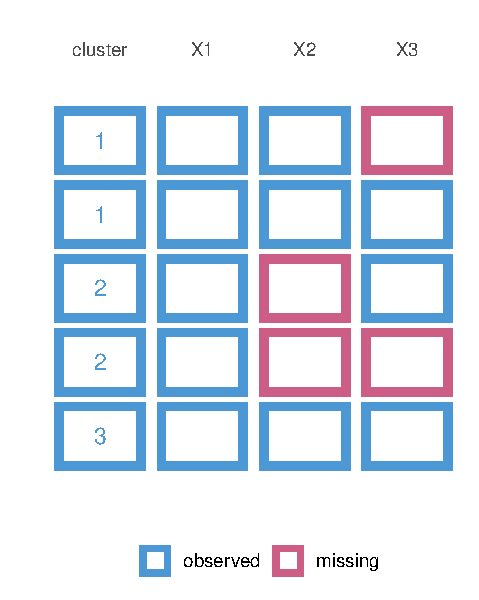
\includegraphics{Manuscript_files/figure-latex/patterns-1} 

}

\caption[Missingness in multilevel data]{Missingness in multilevel data}\label{fig:patterns}
\end{figure}
\end{CodeChunk}

Multilevel data is not spared the ubiquitous problem of missing
information. Just as in single level data, missingness may occur at the
unit level. But with multiple levels of data comes the potential for
missingness at multiple levels. Missingness in multilevel data can be
categorized into two general patterns: systematical missingness and
sporadic missingness, see \citet{resc13}. In figure 1, we show a dataset
with units in the rows and variables in the columns, there are 5 units
nested within 2 clusters, and 3 variables of interest. Variable
\texttt{X1} is completely observed. Variable \texttt{X2} is
systematically missing, \texttt{X3} is sporadically missing.\footnote{Explain
  why.} Systematic missingness can be further subdivided into unobserved
constants (same value per cluster) and non-measured random variables
(which may differ per unit within clusters). In Figure 1, the former
implies that the unobserved values for units 4 and 5 on variable
\texttt{X2} would be equal. With the latter, the values may differ.
Depending on the missing data pattern, there are more or less optimal
way of accommodating the missingness.

Ignoring missing data in research endeavors is almost never a good idea.
Complete case analysis (i.e., excluding all units with one or more
missing entries) can introduce bias in statistical inference and lowers
statistical power. Instead, the missingness should be accommodated
\emph{before} or \emph{within} the analysis of scientific interest.
Especially the former is very generic and popular. Imputing (i.e.,
filling in) the missing values splits the missing data problem from the
scientific problem. The \proglang{R} package \pkg{mice} has become the
de-facto standard for imputation by chained equations, which solves the
missingness one variable at a time, iteratively. \pkg{mice} is known to
yield valid inferences under many different missing data circumstances
\citep{buur18}. In this paper, we'll discuss how to use \pkg{mice} in
the context of multilevel data, under varying missing data
mechanisms.\footnote{Discuss missingness mechanisms before this point,
  add references \citet{yuce08} and \citet{hox15}.}

\hypertarget{aim-of-this-paper}{%
\subsection{Aim of this paper}\label{aim-of-this-paper}}

This papers serves as a tutorial for imputing incomplete multilevel data
with \pkg{mice}. We provide practical guidelines and code snippets for
different missing data situations. For reasons of brevity, we focus on
imputation by chained equations, although JOMO is available in
\pkg{mice} as well. Other useful packages for incomplete multilevel data
include: \pkg{mitml}, \pkg{miceadds}, \pkg{mdmb}.\footnote{Rephrase:
  Some level of knowledge on multilevel models is assumed. We're
  providing an overview of implementations. It's up-to the reader to
  decide which multilevel strategy suits their data. So we won't go into
  detail for the different methods (and equations). Refer to
  \citet{meng94}, an Audigier paper, and a paper by Grund on
  congeniality and random slopes. This paper is just a software
  tutorial. We'll keep it practical.}

We structure this tutorial around three case studies:

\begin{itemize}
\item
  \texttt{mice::popmis} (simulated data on school kids, with MNAR/MAR
  mixture);
\item
  \texttt{metamisc::impact} (real IPD on traumatic brain injuries,
  without \texttt{NA}s);
\item
  \texttt{GJRM::hiv} (simulated patient data on HIV, without
  \texttt{NA}s)
\end{itemize}

For each case study we focus on a different aspect to illustrate how to
impute incomplete multilevel data.

\hypertarget{workflows}{%
\section{Workflows}\label{workflows}}

We introduce three case studies to illustrate the workflow. In the
\texttt{mice::popmis} data, we show the advantages of including the
multilevel structure of the data into the imputation model. In the
\texttt{metamisc::impact} data we'll show how to induce missingness and
solve it in real-world data. In the \texttt{GJRM::hiv} we provide novel
methodology\footnote{not really, the methods exist already, but how to
  show that this is something new and exciting?} for imputing MNAR
missingness according to the Heckman model.

For each case study we'll look at least at: 1) the incomplete data; 2)
the imputation model; 3) the imputed data; and 4) how to obtain pooled
estimates for the analysis of scientific interest.

\hypertarget{case-study-i-popularity}{%
\subsection{Case Study I: Popularity}\label{case-study-i-popularity}}

\texttt{popNCR} is a simulated dataset with pupils clustered in classes,
\(n_{\text{participants}} = 2000\), \(n_{\text{clusters}} = 100\), on 7
variables:

\begin{itemize}
\tightlist
\item
  \texttt{pupil} Pupil number within class,
\item
  \texttt{class} Class number,
\item
  \texttt{extrav} Pupil extraversion,
\item
  \texttt{sex} Pupil gender,
\item
  \texttt{texp} Teacher experience (years),
\item
  \texttt{popular} Pupil popularity,
\item
  \texttt{popteach} Teacher popularity.
\end{itemize}

\hypertarget{incomplete-data}{%
\subsubsection{Incomplete data}\label{incomplete-data}}

\begin{CodeChunk}
\begin{figure}

{\centering 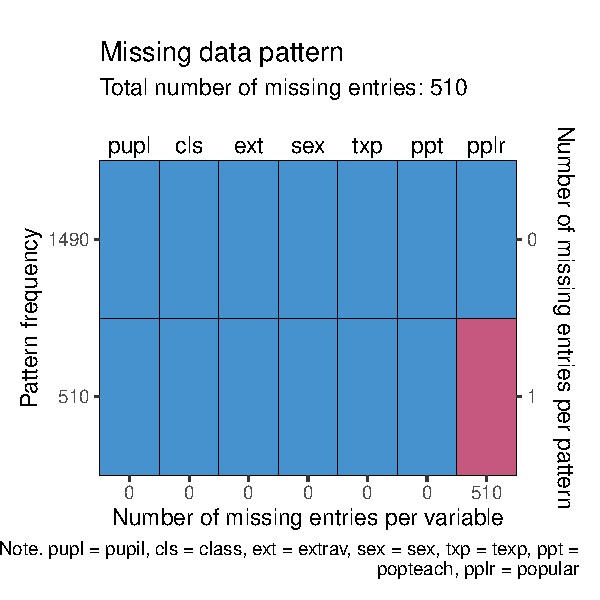
\includegraphics{Manuscript_files/figure-latex/pop_pat-1} 

}

\caption[Missing data pattern in the popularity data]{Missing data pattern in the popularity data}\label{fig:pop_pat}
\end{figure}
\end{CodeChunk}

The popularity data is created such that there are strong relations
between the incomplete variables and the clustering variable
\texttt{class}. We can express this using the intra-class correlation
(ICC). For \texttt{popular} the ICC is 0.33. For \texttt{popteach} it is
0.31. It would thus be wise to use multilevel modeling.

The missingness in this dataset is induced conform MAR and MNAR
mechanisms. The missing data pattern, Figure \ref{fig:pop_pat}, shows
the systematic nature of the missingness.

To develop the best imputation model, we need to know whether the
missingness in one variable depends on the observed values of other
variables. Visual inspection usually suffices. We'll highlight only two
variables to illustrate, but ideally one would inspect all relations.
The questions we'll ask are: `Does the missing data of \texttt{popular}
depend on \texttt{popteach}?' and `Does the missingness in teacher
popularity depend on pupil popularity?' We'll evaluate this by making a
histogram of \texttt{popteach} separately for the pupils with known
popularity and missing popularity, and the other way around.

In Figure \ref{fig:pop_dist} we see that the distribution for the
missing \texttt{popular} is further to the right than the distribution
for observed \texttt{popular}. This would indicate a right-tailed MAR
missingness. In fact, this is exactly what happens, because the
missingness in these data was created manually. Now, we've made it
observable by examining the relations between the missingness in popular
and the observed data in \texttt{popteach}. There is also a dependency
between the missingness in teacher popularity and pupil popularity. The
relation seems to be right-tailed as well.

\begin{CodeChunk}
\begin{figure}

{\centering 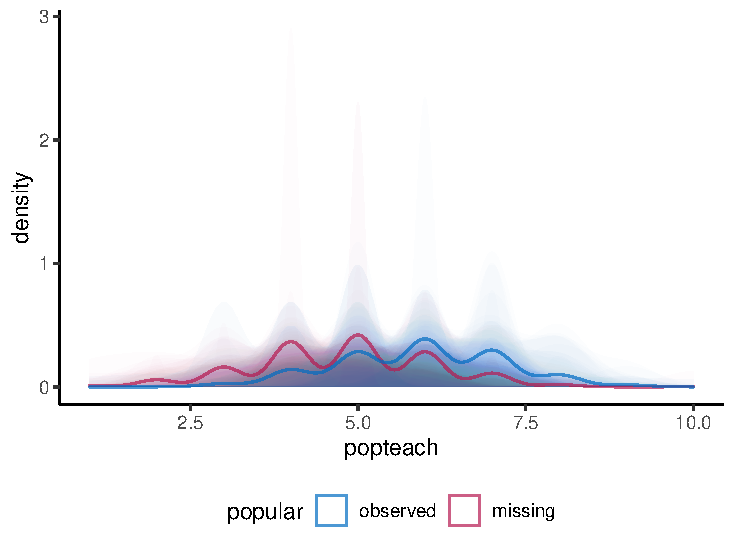
\includegraphics{Manuscript_files/figure-latex/pop_dist-1} 

}

\caption[Conditional distributions in the popularity data]{Conditional distributions in the popularity data}\label{fig:pop_dist-1}
\end{figure}
\begin{figure}

{\centering 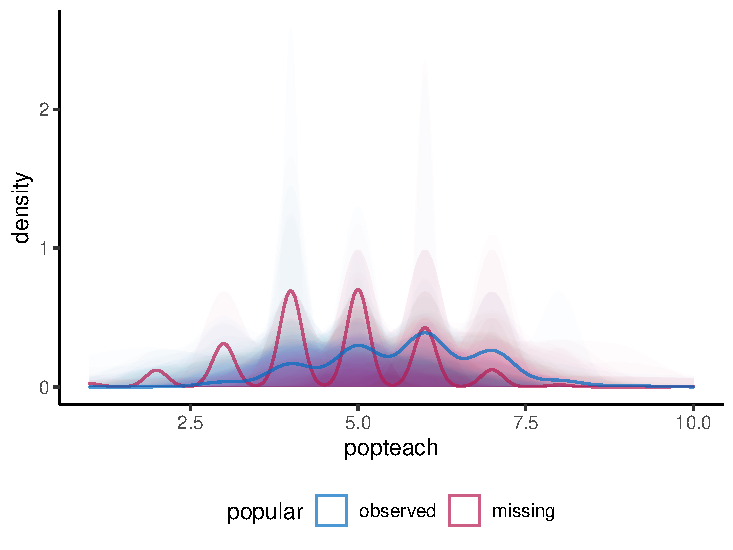
\includegraphics{Manuscript_files/figure-latex/pop_dist-2} 

}

\caption[Conditional distributions in the popularity data]{Conditional distributions in the popularity data}\label{fig:pop_dist-2}
\end{figure}
\end{CodeChunk}

\hypertarget{imputation-model}{%
\subsubsection{Imputation model}\label{imputation-model}}

The first imputation model that we'll use is likely to be invalid. In
this model, we ignore the multilevel structure of the data, despite the
high ICCs. This is purely to illustrate the effects of ignoring the
clustering in our imputation effort.

We'll use predictive mean matching to impute the continuous variables
and logistic regression to impute the binary variable \texttt{sex}. We
do not use the observation identifier \texttt{pupil} or cluster
identifier \texttt{class} as predictors to impute other variables.

\begin{CodeChunk}
\begin{CodeInput}
R> # dry run to get imputation parameters
R> ini <- mice(pop, maxit = 0)
R> 
R> # extract predictor matrix and adjust
R> pred <- ini$pred
R> pred[, c("class", "pupil")] <- 0
R> 
R> # impute the data, ignoring the cluster structure
R> imp_ignored <- mice(pop, maxit = 10, pred = pred, print = FALSE)
\end{CodeInput}
\end{CodeChunk}

\hypertarget{imputed-data}{%
\subsubsection{Imputed data}\label{imputed-data}}

\begin{CodeChunk}


\begin{center}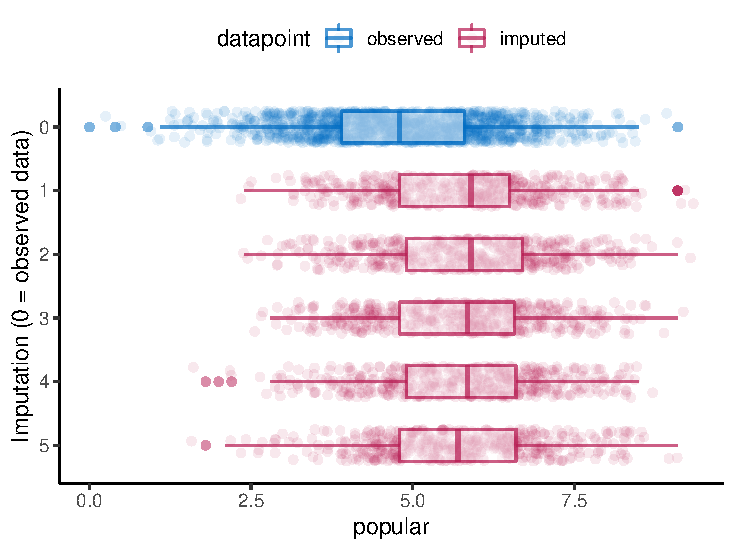
\includegraphics{Manuscript_files/figure-latex/pop_ignored_eval-1} \end{center}

\begin{CodeOutput}
      vars incomplete   ignored
1  popular  0.3280070 0.2958571
2 popteach  0.3138658 0.2561198
3     texp  1.0000000 0.4696024
\end{CodeOutput}
\end{CodeChunk}

As the original ICCs show, 100\% of the variance in \texttt{texp} can be
attributed to the clustering variable \texttt{class}. This tells us that
the multilevel structure of the data should be taken into account. If we
don't, we'll end up with incorrect imputations, biasing the effect of
the clusters towards zero.

We can also observe that the teacher experience increases slightly after
imputation. This is due to the MNAR missingness in \texttt{texp}. Higher
values for \texttt{texp} have a larger probability to be missing. This
may not a problem, however, if at least one pupil in each class has
teacher experience recorded, we can deductively impute the correct
(i.e.~true) value for every pupil in the class.

\hypertarget{imputation-model-1}{%
\subsubsection{Imputation model}\label{imputation-model-1}}

We'll now use \texttt{class} as a predictor to impute all other
variables. This is still not recommended practice, since it only works
under certain circumstances and results may be biased. But at least, it
includes some multilevel aspect. Colloquially, this is `multilevel
imputation for dummies'.

\hypertarget{imputed-data-1}{%
\subsubsection{Imputed data}\label{imputed-data-1}}

\begin{CodeChunk}


\begin{center}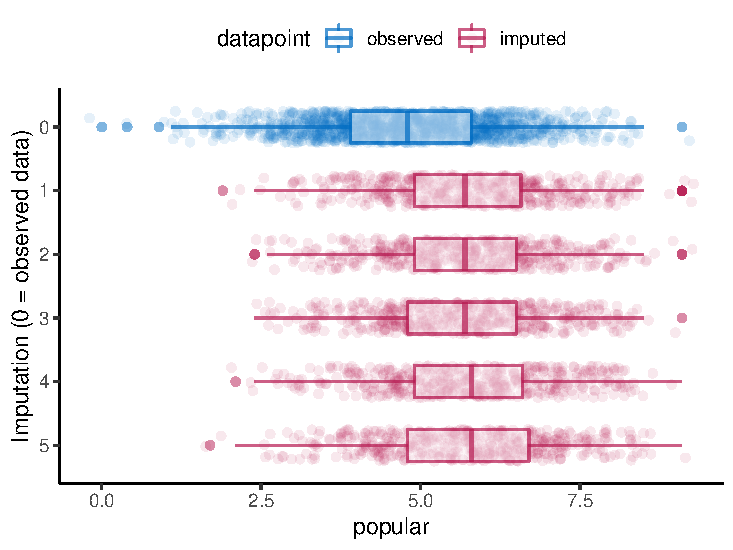
\includegraphics{Manuscript_files/figure-latex/pop_predictor_eval-1} \end{center}

\begin{CodeOutput}
      vars incomplete   ignored predictor
1  popular  0.3280070 0.2958571 0.3581435
2 popteach  0.3138658 0.2561198 0.3446899
3     texp  1.0000000 0.4696024 1.0000000
\end{CodeOutput}
\end{CodeChunk}

Now, we can clearly see that the imputed values of \texttt{texp} are
higher than the observed values, which is in line with right-tailed
MNAR.

The ICCs are way more in line with the ICCs in the incomplete data. But
this is a quick and dirty way of imputing multilevel data. We
\emph{should} be using a multilevel model.

\hypertarget{imputation-model-2}{%
\subsubsection{Imputation model}\label{imputation-model-2}}

To include\ldots{}

\hypertarget{case-study-ii-impact}{%
\subsection{Case study II: IMPACT}\label{case-study-ii-impact}}

\texttt{impact} is traumatic brain injury data with patients clustered
in studies, \(n_{\text{participants}} = 11022\) and
\(n_{\text{clusters}} = 15\), on the following 11 variables:

\begin{itemize}
\tightlist
\item
  \texttt{name} Name of the study,
\item
  \texttt{type} Type of study (RCT: randomized controlled trial, OBS:
  observational cohort),
\item
  \texttt{age} Age of the patient,
\item
  \texttt{motor\_score} Glasgow Coma Scale motor score,
\item
  \texttt{pupil} Pupillary reactivity,
\item
  \texttt{ct} Marshall Computerized Tomography classification,
\item
  \texttt{hypox} Hypoxia (0=no, 1=yes),
\item
  \texttt{hypots} Hypotension (0=no, 1=yes),
\item
  \texttt{tsah} Traumatic subarachnoid hemorrhage (0=no, 1=yes),
\item
  \texttt{edh} Epidural hematoma (0=no, 1=yes),
\item
  \texttt{mort} 6-month mortality (0=alive, 1=dead).
\end{itemize}

The data is already imputed (Steyerberg et al, 2008), so we'll induce
missingness ourselves. For example, MAR missingness varying by
cluster.\footnote{Observed data pattern should differ per cluster. So,
  in cluster 1, the missingness would depend on age, but not in cluster
  two. Split the dataframe and run \texttt{ampute()} on each cluster.}

\hypertarget{pooling}{%
\subsection{Pooling}\label{pooling}}

\begin{itemize}
\item
  Analysis of scientific interest.
\item
  Pooling using \texttt{mitml}.
\item
  Pooling `regular' parameters vs more `exotic' parameters (SE of
  residual errors, or autocorrelation)
\end{itemize}

\hypertarget{discussion}{%
\section{Discussion}\label{discussion}}

\begin{itemize}
\item
  JOMO in \pkg{mice} -\textgreater{} on the side for now
\item
  Additional levels of clustering
\item
  More complex data types: timeseries and polynomial relationship in the
  clustering.
\end{itemize}

\hypertarget{think-about}{%
\section{Think about}\label{think-about}}

\begin{itemize}
\item
  Adding some kind of help function to mice that suggests a suitable
  predictor matrix to the user, given a certain analysis model.
\item
  Adding a \texttt{multilevel\_ampute()} wrapper function in mice.
\item
  Exporting \texttt{mids} objects to other packages like \texttt{lme4}
  or \texttt{coxme}?
\end{itemize}

\renewcommand\refname{References}
\bibliography{../References/multilevelmice.bib}


\end{document}
